%% how will i tackle the problem with justifications 
%% based on ideas in BACKGROUND
\newcommand{\liam}[1]{$\langle$ \textit{\textbf{Liam} #1} $\rangle\ $}
\chapter{Implementation}\label{ch:impl}

\section{Using a MATLAB-based neural network as reference} \label{se:impl.matlab.nn}

\liam{You should start off by mentioning and citing the specific Matlab implementation you're referring to, if you don't do so in your introduction.}
There are several motivations for choosing this particular implementation of a neural network in MATLAB as a starting point. Firstly, the MATLAB implementation clearly shows the mathematical structure of a neural network, succinctly expressing the matrix multiplication and vectorisation operations out of which a neural network is built. It was projected that, seeing as high level matrix operations can also be easily expressed in Accelerate, this implementation would be reasonably simple to adapt, and the closest-in-spirit to an Accelerate implementation.

Secondly, the MATLAB implementation also included a data set with expected answers to which I can compare my own implementations. Thus, I could be assured that my implementation in Accelerate was accurate enough to be reliable, particularly in the light of the difficulty of debugging Accelerate programs. Passing this accuracy test will indicate that my small network is reliable enough to be built upon in future machine learning developments.

Thirdly, the codebase on which I am basing my implementation is from Coursera, an online course service, specifically the Machine Learning course made by Andrew Ng of Stanford University. This course has drawn wide praise for its material and presumed to be reviewed by many in the same field. The structure of the course is reliable in terms of correctness and efficiency, and implemented already in a manner that is idiomatic for the Machine Learning community. Hence, I projected that the MATLAB implementation would be optimised for the best performance.

Lastly, in terms of familiarity, I was more conversed with MATLAB than with other neural network implementations, such as Python, C++, or Haskell, (PUT REFERENCES TO THESE IMPLEMENTATIONS) and as such I could avoid needlessly increasing the time to start the project by choosing a language I was already comfortable using and an implementation I had already studied. While researching other implementations, I found that it took more time to understand these as I had to additionally learn the language in enough detail to understand the code being written, and the implementations differed in many details from the versions with which I was familiar.

TO CHECK::::: Can C++ or Python versions use multiple threads/GPU?

\subsection{Key differences from Accelerate} \label{se:impl.matlab.background}
%% or divide this up into implementation section

MATLAB, or Matrix Laboratory, is a highly doman-specific programming language, specialised to conduct numerical calculations and analysis. It was created in the 1970s, and is an imperative procedural language with a wide array of built in linear algebra operations. It is widely used among the industry and academia, particularly in science, engineering and economics.

MATLAB is also dynamically typed, meaning that the types may change during runtime. Futhermore, it is described as a weakly typed programming language, in that types are implicitly converted whenever 
a mismatch occurs.

MATLAB functions automatically apply multiplications of a scalar term to a matrix, by applying the operation of the scalar to each element of the matrix. Thus, if \texttt{a} is a scalar and \texttt{xs} is a matrix, it is possible to simply do \texttt{a} $\times$ \texttt{xs}. In Accelerate, this would be \texttt{A.map (*a) xs}. As a result, MATLAB code is deceptively compact --- it may not reveal the actual structure of the underlying operation just from a surface examination of the program syntax. 

Other notable differences from other languages include the starting index of matrices and arrays being $1$, not $0$.
\liam{This next sentence about dispatching doesn't make sense to me. Also, you don't use the OO features of Matlab so perhaps just don't mention it at all} Also, MATLAB method dispatching does not strictly adhere to the method signature, but selects the appropriate method by first matching the arguments in a class precedence and then by left-most priority~\cite{Mat17}. %MATLAB does not support overloading functions of the same name using different signature of the same name.

\section{Accelerate Implementation} \label{se:impl.acc}

\subsection{Neural network structure} \label{se:impl.nn.struct}

I have implemented a two-layered, fully connected simple neural network, with one hidden layer.

My implementation can easily be modified to take more than 1 hidden layer by changing the \texttt{nnCostFunction}. For instance, each extra hidden layer should only require the addition of two matrix multiplications in the feed-forward and backpropagation components, as well as the necessary steps to update the theta layer (see~\ref{fig:nnCostFunction.hiddenlayers}).

\begin{figure}
  \begin{lstlisting}
    -- current feed-forward with 1 hidden layer
    a3 :: Acc (Matrix Float)
    a1 = xs 
    z2 = theta1 <> transpose a1 
    a2 = (fill (lift (Z :. h :. constant  1)) 1 :: Acc (Matrix Float)) 
         A.++ (A.transpose $ A.map sigmoid z2) 
    z3 = a2 <> A.transpose theta2 
    a3 = A.map sigmoid z3
    
    -- an example feed-forward with 2 hidden layers
    a4 :: Acc (Matrix Float)
    a3' = (fill (lift (Z :. h' :. constant  1)) 1 :: Acc (Matrix Float))
          A.++ (A.transpose $ A.map sigmoid z3)
    z4 = a3' <> A.transpose theta3
    a4 = A.map sigmoid z4
    
    -- an example backpropagate with 2 hidden layers
    d4 = A.zipWith (-) a4 ys
    d3 = A.zipWith (*) 
         (d4 <> theta3)
         ((fill (lift (Z :. h' :. constant  1)) 1 :: Acc (Matrix Float)) 
           A.++ (A.transpose $ A.map sigmoidGradient z3)) 
    d2 = A.zipWith (*) 
         (d3 <> theta2)
         ((fill (lift (Z :. h :. constant  1)) 1 :: Acc (Matrix Float)) 
           A.++ (A.transpose $ A.map sigmoidGradient z2)) 
  \end{lstlisting}
  \caption{Changing the number of hidden layers in \texttt{nnCostFunction}}
  \label{fig:nnCostFunction.hiddenlayers}
\end{figure}

\subsection{Program structure} \label{se:impl.program.struct}

In terms of program structure, I closely followed the control flow of the MATLAB version. It can be partitioned into three main subroutines: (1) initialisation; (2) the neural network cost function; and, (3) function minimisation via the conjugate gradient method. The implementation code is available at~\cite{McDJeo}.

\subsubsection{Initialisation} \label{se:impl.init}

Initialisation is a straightforward process. We initialise (1) the regularisation parameter \texttt{lambda}; (2) initial weight vectors, in this instance \texttt{theta1} and \texttt{theta2}; (3) size of the input, hidden, output layers; and, (4) the input training data set \texttt{xs} and the output vector \texttt{ys} to conduct the supervised learning. 

The number of input units correspond to the number of attributes in each sample of \texttt{xs}, whereas the output units correspond to the number of classifications that these samples could be divided into, or, the range of the values of \texttt{ys}. Setting the number of neurons in the hidden layer is mostly done by a mixture of guesswork and trial-and-error. In \ref{se:res.testdata}, 25 and 300 neurons comprise the hidden layer for two different data sets of handwritten numbers. These sizes were taken from other implementations with the same data sets, who had found these the most effective numbers by testing.

The matrix \texttt{xs} represents $m$ training set data. After it has been loaded, each row of \texttt{xs} should represent a single training example, $x_1, x_2, ..., x_m$ where the length of vector $x_i$ is the size of the input layer. A column vector of $1$s is added to the leftmost of the array to represent the bias neuron, as shown below.
\[
 \texttt{xs} =
    \begin{bmatrix}
      1 \\
      1 \\
      ... \\ 
      1
    \end{bmatrix}
    \begin{bmatrix}
       x_1 \\
       x_2 \\
       ... \\
       x_m
    \end{bmatrix}
\]

This is implemented in Accelerate using a combination of \texttt{fill} and concatenation \texttt{A.++}. Accelerate's operations are not the same as Haskell Prelude's, even if some operation names coincide. Thus they are distinguished by a qualified import: \texttt{A}, \texttt{P} for Accelerate and Prelude correspondingly, for instance \texttt{A.++} and \texttt{P.++}. Other key array manipulation functions used throughout the program include \texttt{A.take, A.drop, A.map} and \texttt{A.zipWith}.

The effectiveness of the random initialisation of weight vectors will influence the accuracy of the neural network. Initial values should be in the range $[-\epsilon_{init}, \epsilon_{init}]$~\cite{Ng12}. One popular choice of $\epsilon_{init}$ is,
\[ \epsilon_{init} = \sqrt{\frac{6}{L_{in} + L_{out}}} \]
where $L_{in}$ is number of units in the preceding layer, and $L_{out}$ is the number of units in the subsequent layer of the weight vector-in-question. 

The optimal regularisation parameter \texttt{lambda} is also discovered by trial-and-error. It is set by the user to determine the level of fitting of the neural network to the training set is considered `overfitting'. Whether higher or lower overfitting to the training set is better or worse for making predictions on new samples depends entirely on the nature of the data. 

\subsubsection{Neural network cost function, \texttt{nnCostFunction}} \label{se:impl.nnCostFunction}

This function applies both the feed-forward and back-progapation to sample data inputs and updates the weight vectors and error costs accordingly. 

As described in \ref{sec:training} we apply the BGD method by grouping all the sample data into one large batch, passing them in all at once, for higher accuracy. 

As the \texttt{nnCostFunction} is used in conjunction with the \texttt{fmincg} function (\ref{se:impl.fmincg}), it was necessary to flatten all the weight vectors into a single dimension before passing them into, and returning them from the \texttt{nnCostFunction}. The flattened vector is sliced and reshaped to restore the vectors to their original shapes inside \texttt{nnCostFunction}, implemented via the Accelerate \texttt{reshape} function as shown in~\ref{fig:reshape}.

\begin{figure}
	\begin{lstlisting}
	-- type of reshape
    reshape :: (Shape sh, Shape sh', Elt e) =>
                Exp sh -> Acc (Array sh' e) -> Acc (Array sh e)

    -- unroll theta1, theta2
    theta1 = reshape (index2 hiddenl (inputl +1)) $ A.take (hiddenl*(inputl+1)) thetas
    theta2 = reshape (index2 outputl (hiddenl+1)) $ A.drop (hiddenl*(inputl+1)) thetas
	\end{lstlisting}
  	\caption{Reshaping vectors into matrices in Accelerate.}
	\label{fig:reshape}
\end{figure}

Using \texttt{reshape} can be initially cumbersome, because it must be supplied with an \texttt{Exp} of the output shape. This can be supplied in various ways, and may require its type to be explicitly specified. For example, in the case where one \texttt{lift}s a \texttt{(Z:.m:.n)} expression to supply \texttt{fill} with an \texttt{Exp (Z:.Int:.Int)}, a type signature is required:
$$\texttt{fill (lift (Z:.m:.n)) 1 :: Acc (Matrix Float)}$$
Thus, I found operations involving shape parameters quite tricky at times due to the necessity of explicit typing.

Matrix multiplications was initially implemented using \texttt{mmult}, but to improve performance on the CPU LLVM backend, the foreign function interface of Accelerate \liam{cite rob here} was used to call the matrix multiplication function from the \texttt{hmatrix} package, which has a better performance. 

\subsubsection{Function minimisation via conjugate gradient method, \texttt{fmincg}} \label{se:impl.fmincg}
 Generally, function minimisation by conjugate gradients is a quadratically convergent gradient method used to locate a local minimum when the function has several variables, or, is \textit{multivariate}~\cite{FleRee}. This function repeats \texttt{nnCostFunction}, a multivariate function, for certain number of iterations, and progressively tries to minimise the error in the weight matrices.

In MATLAB, function minisation by conjugate gradient is a function called \texttt{fminunc}, which states that given a starting point \texttt{x0} (can be a scalar, vector or a matrix), \texttt{x} is the the local minimum of unconstrained function \texttt{func}~\cite{Mat17}:
$$\texttt{x = fminunc(func, x0)}$$
\texttt{fmincg} function is a modified version of \texttt{fminunc} and has the following MATLAB equation:
$$\texttt{function [X, fX, i] = fmincg(f, X, options, P1, P2, P3, P4, P5)}$$
According to the author, it is more efficient than \texttt{fminunc} in that it uses `Polack-Ribiere' conjugate gradients, quadratic and cubic polynomial approximations and the `Wolfe-Powell stopping criteria' to more efficiently calculate slope and stepping sizes~\cite{Reb13}. The mathematics behind this method is beyond the scope of my understanding.

The \texttt{fmincg} function terminates when it either finds the local minimum, or if the progress is so insignificant that it is not worth any further exploration. It must be given a cost function \texttt{f}, initial weight vector \texttt{X} and maximum iteration number in \texttt{options}. Other parameters are not supplied. 

The function returns the solution vector as \texttt{X} and a cost vector as \texttt{fX}. \texttt{fX} starts off as an empty vector, and \texttt{fmincg} pushes the cost/error of the newly recalibrated weights in each iteration to the back of \texttt{fX}. The end result is that the caller can see the progress made throughout the iterations by checking \texttt{fX}. Other variables are discarded.

The Haskell/Accelerate type signature of \texttt{fmincg} can be seen in~\ref{fig:fmincg}. The vector argument is a concatenation of flattened weight matrices and is fed into the function argument. This is to enable \texttt{fmincg} to execute the function independently from the structure of the underlying neural network, i.e. the number of hidden layers. It is a artifact of MATLAB methodology that needs better implementation in Accelerate (see Chapter~\ref{ch:eval}).

\begin{figure}
	\begin{lstlisting}
	fmincg :: (Acc (Vector Float) -> Acc (Scalar Float, Vector Float))
           -> Acc (Vector Float)
           -> (Acc (Vector Float), Acc (Vector Float))
	\end{lstlisting}
  	\caption{Function minimise conjugate gradient function.}
	\label{fig:fmincg}
\end{figure}

I faced a couple of challenging factors in implementing this function. First, the MATLAB version had approximately 17 parameters, most of which are overwritten and interact in complex, intricate ways. Without a knowledge of the underlying mathematics, I could not fully comprehend the overall structure of this 175-line procedure. The ambiguity and similarity of parameter names, such as \texttt{d1, d2, d3, f1,..., v1,...}, did nothing to ease the problem. 

Secondly, it is difficult to follow the flow of control in \texttt{fmincg}. In order to reduce the chance of errors arising, I chose to initially follow the procedure very closely, hoping to optimise incrementally later. Certain expressions were substituted where operations had not yet been implemented in Accelerate (see~\ref{se:impl.limits}). Additionally, I could not model the extremely complex flow control perfectly, and the known issues and bugs are mentioned in~\ref{se:impl.limits}.

Thirdly, MATLAB \texttt{fmincg} was composed of three \texttt{while} loops within each other and three \texttt{if-else} statements, one of the latter which resulted in a flow divergence. The last factor in particular may have greatly reduced this implementation's suitability for GPU execution, as such parallelism with flow divergence may can cause drastic problems in GPU performance, which favours non-divergent \emph{flat-data parallelism}, where sequential operations can be applied in parallel over bulk data.

On the positive side, the flow divergence is only triggered upon a failure to find a local minimum; which, according to~\cite{Reb13} occurs when the function supplied to \texttt{fmincg} is inaccurate or unsuitable. For this particular implementation, I have taken the assumption that the function supplied, \texttt{nnCostFunction} is accurate and that there is always a local minimum that \texttt{fmincg} will find. In my limited tests (see Chapter~\ref{ch:results}), all results support this assumption. More broadly, the correctness of the function can be checked for prior to being supplied to \texttt{fmincg}.

To make my implementation more manageable, I divided the MATLAB code into their \texttt{while} loops. These were implemented using Accelerate's \texttt{awhile} flow control combinator. 

This combinator \texttt{awhile} requires variables that change during the loop and/or are returned when function ends, to be wrapped into a single \texttt{Acc} tuple to be used for the loop process. The functions \texttt{lift} and \texttt{unlift} are necessary to pack and unpack the variables respectively in each loop, for condition checks and for loop execution. An interesting fact I learnt was that Haskell's type inference quickly meets its match with Accelerate --- it cannot infer the types of some variables unless they are unambiguously used after an \texttt{unlift} call. It is thus sometimes necessary to specify types of certain terms to assist Haskell with type inference as seen in~\ref{fig:unlift}.

\begin{figure}
	\begin{lstlisting}
    d1, f1, limit :: Acc (Scalar Float)
    m :: Acc (Scalar Int)
    (theta, df2, d1, d2, d3, f1, f2, f3, z1, z2, z3, m, limit) = unlift $ awhile cond body initial
	\end{lstlisting}
  	\caption{Assisting Accelerate by specifying types of unused variables in \texttt{unlift}.}
	\label{fig:unlift}
\end{figure}

\section{Known bugs} \label{se:impl.limits}

There are several issues with my Accelerate implementation. One, it does not have the robust failure handling, allowing it withstand incorrect inputs analogously to the MATLAB programs. For instance, I have already mentioned in \ref{se:impl.fmincg} that the function supplied to \texttt{fmincg} must have a clear minimum. 

Also, there are cases in \texttt{fmincg} where some variables need to checked for \texttt{isinf}, \texttt{isreal} or \texttt{isnan}, that is, be checked for an infinity, a real number, or 'not-a-number' floating-point properities, correspondingly. As these functions are not yet available in Accelerate, I substituted them for expressions which I believe will cover those particular situations. For instance, \texttt{isreal} check may arise when a determinate may be less than zero; \texttt{isnan} may arise when a divisor is zero. I was not able to devise a check for \texttt{isinf}, however, so the implementation may not cover all the range of inputs and remain fault-free.

Secondly, MATLAB's \texttt{double} is by default a double-precision data type, and requires 64 bits~\cite{Mat17}. Yet, after testing it on the sample data, importing the values in Accelerate as \texttt{Double}s produces a result further away from the MATLAB result than when I pass them to Accelerate as \texttt{Float}s. Not only that, the accuracy of the Accelerate neural network predictions after training decreased with the same training set when the data was passed as a \texttt{Double}. 

The source of the inaccuracy may be due to \texttt{fmincg}. There is one line that seems to account for overflow, by subtracting \texttt{realmin} from a dividend as seen in~\ref{fig:realmin}. The value \texttt{realmin} for a \texttt{float} is defined as $1.1755e^{38}$ and for a \texttt{double} is $2.2251e^{308}$ in MATLAB. These different by orders of magnitude ($1xe^{270}$) and could vastly affect the result. In my implementation, I have currently taken out \texttt{realmin} from the equation, which increases the risk of division by zero but does not seem to be problematic in practice.

\begin{figure}
	\centerline{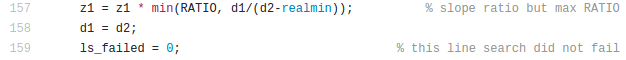
\includegraphics[width=\linewidth]{realmin.png}}
	\caption{MATLAB's \texttt{double} is actually a \texttt{float}? What it means for \texttt{realmin}.}
	\label{fig:realmin}
\end{figure}

Lastly, some of the optimisations in \texttt{fmincg} has been ignored, namely: (1) the innermost and middle loop iterations, thus the loop counter \texttt{M} is set to 1; and, (2) the handling of a failure case. The reason for (2) has already been discussed in \ref{se:impl.fmincg}. For (1), testing has shown that the iterations other than exactly once for the sections in question produces erroneous results, and the reasons for this is unfortunately still unknown at the time of writing. In addition, although setting \texttt{M=1} seems to closely align my program's results to MATLAB's results in the first training set, my neural network was unable to yield as high accuracy rate as in ~\cite{LeC98} for the second training set, deviating by almost 10 per cent (see Chapter~\ref{ch:results}).

\section{Other works}
I have also implemented a logistic regression cost function, which is akin to a neural network without any hidden layers. This can be accessed at ~\cite{McDJeo}. This function produces analogous results to the equivalent MATLAB implementation.
